\section{Introduction}
The brewery Refslevbæk Bryghus A/S recently won the “best beer of the year” 
award, which has led to an increase in demand for their products. Before this
increase, every product was made in smaller batches. However, their current
production line does not fulfil these demands. This has led them to purchase a
new, bigger brewing machine. So far, the brewing has involved a lot of manual
processes. The brewery now needs a Manufacturing Execution System, MES,
developed that implements a large degree of automation and enables a more
efficient beer production. \\

% maybe just f****** delete this sh*t
% As students, this project gives the group great learning experience as
% well as a good idea of how the development of such a system would take place. 
% During the project, the group will learn how to create and set up an Open
% Platform Communications Unified Architecture, OPC-UA, client, and how to make it
% communicate directly to a physical machine. The group will learn to host a web
% server, from which the machine can be controlled, and access it as a website.
% The group will also have the chance to learn and use a new scripting language,
% JavaScript.

\subsection{Problem Statement}
In Table \ref{table:problem-statement-report}, the finished problem, the problem
statement, and related questions are listed.
\begin{table}[ht]
    \captionof{table}{Problem statement showcase}
    \begin{tabularx}{\textwidth}{|>{\RaggedRight}p{4cm}|>{\RaggedRight}X|}
        \hline
        \textbf{Problem} & The current production line is not efficient enough to keep up with the demand of the beer, while still maintaining a high-quality product. \\
        \hline
        \textbf{Problem Statement} & How to apply an MES to control and optimise the brewing process at Refslevbæk Bryghus A/S, to maximise the production of high-quality beer. \\
        \hline
        \textbf{Related questions} & 
            \begin{itemize}
                \item How can the production be optimised?
                \item How can calculus and linear algebra be utilised, to provide a meaningful overview of the production line?
                \item How can a web based frontend for the MES be created?
                \item How can the different aspects of the system be separated? (separation of concerns).
            \end{itemize} \\
            \hline
    \end{tabularx}
    \label{table:problem-statement-report}
\end{table} 

\subsection{Overview of project}
This project aims to improve the beer production line by increasing quantity
while maintaining quality. To accomplish this, the chosen solution will offer
an interactive web interface for monitoring, controlling and adjusting the
brewery machine. This is done by having the web interface interact with a REST
API that connects to a client. This client controls the machine through an
OPC-UA server connection and stores relevant data in a database through the API.

\subsection{Objectives}
The group wants to create a dashboard solution that controls and gets the
necessary information from the brewery machine, to display information about the
current - and previous - batches.\\

The group wants to host the REST API and Website on a Linux based server on a
fully qualified domain name using the container technology Docker which should
be configured via Docker Compose. Furthermore, the group aims to set up a
continuous integration pipeline for development via GitHub Actions (makes it
easy to automate software workflows) and continuous delivery via Watchtower (an
automatic deployment tool).

\subsection{Solutions}
\begin{figure}[h]
\centering 
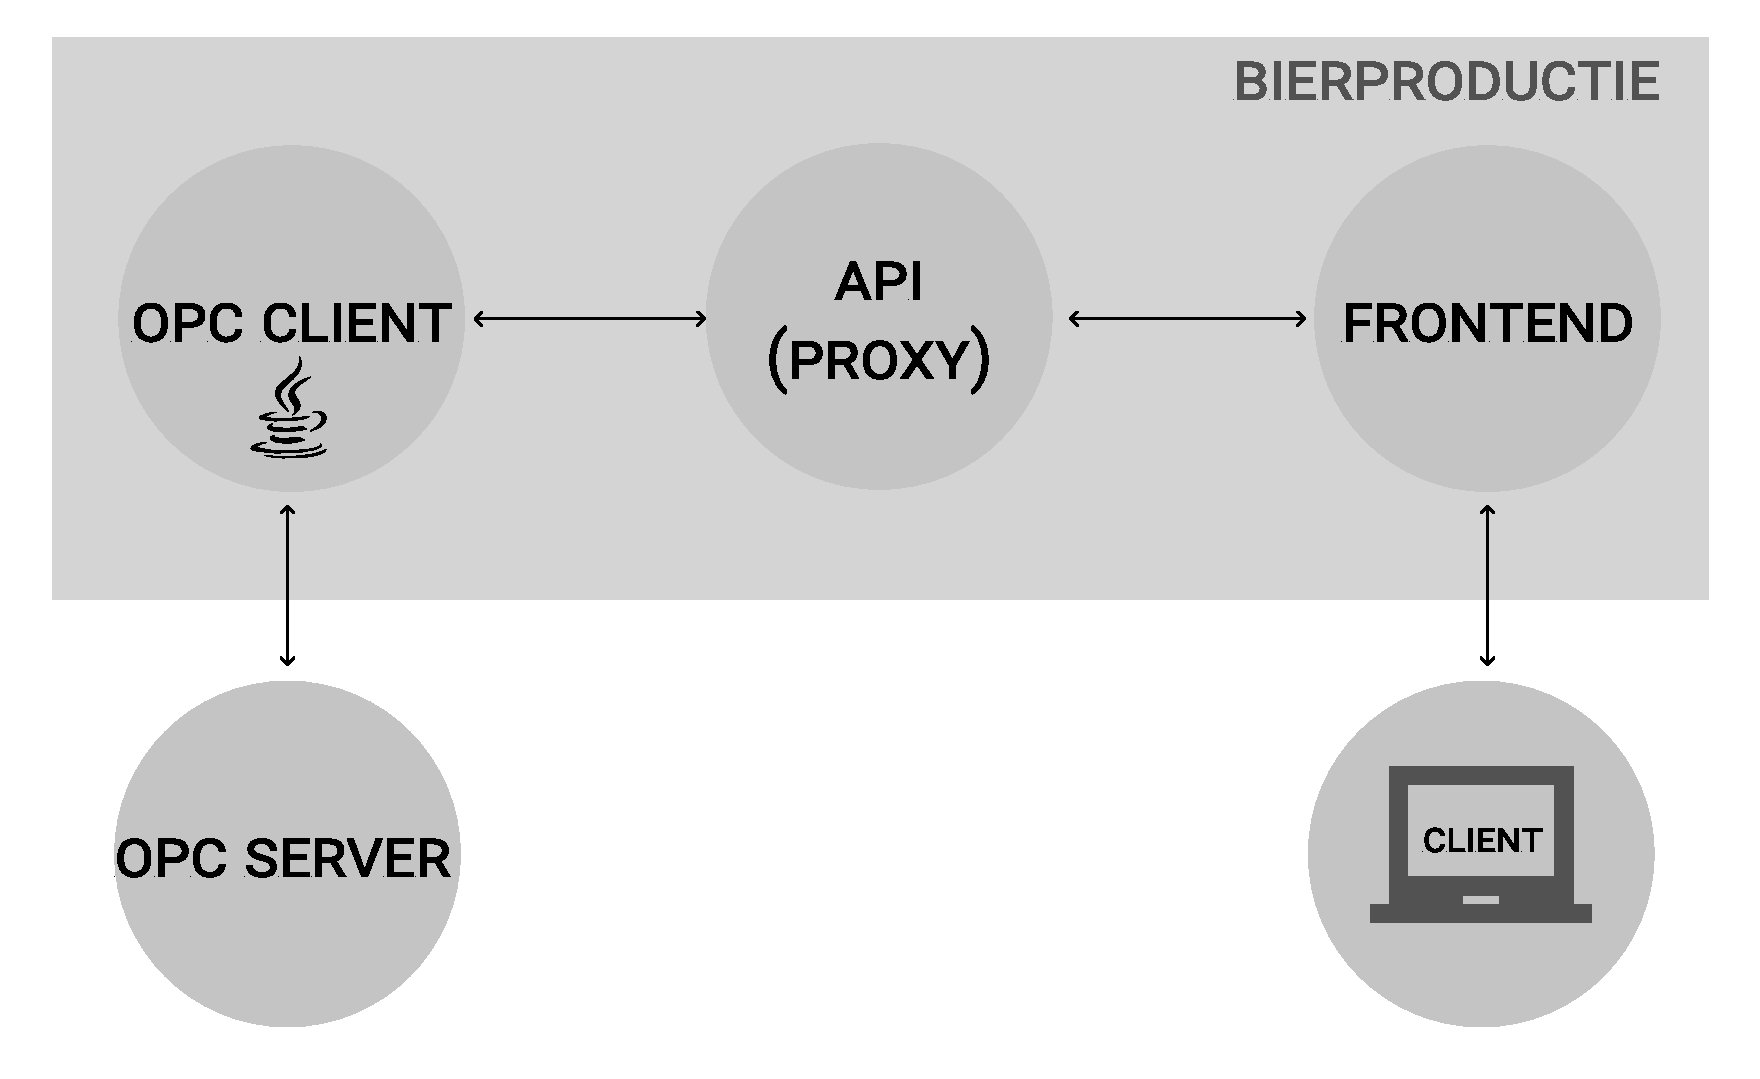
\includegraphics[scale=0.3]{../project_proposal/images/system_drawing.pdf}
\caption{System drawing} 
\label{figure:system_drawing}
\end{figure}

The distributed system consists of five sub-systems as seen in Figure
\ref{figure:system_drawing}, \textit{OPC-Server}, \textit{OPC-Client},
\textit{REST API}, \textit{Dashboard} and the Client Computer. The Bierproductie
project consists of three of these systems, namely: \textit{OPC-Client},
\textit{REST API} and \textit{Dashboard}. The group will be developing these
three.

\subsubsection{OPC-UA Client}
The OPC-UA client is responsible for communicating with the brewing machine via
the OPC-UA server. This is needed to send and receive data via
commands.

\subsubsection{Website}
The website user interface is where the client will be able to interact with
the system. The website will enable the user to control, monitor and adjust
the brewing machine. Live relevant data will also be collected, displayed and
can be shown on the dashboard.

% The subsubsection Website is not very detailed. It would be nice to know how 
% a user would interact with the system. What kind of “functionality” will the 
% remote interface contain?

\subsubsection{REST API}
The REST API functions primarily as a gateway in this design, handling the
communication between the client and the dashboard. For the
dashboard to receive data via fetch calls in JavaScript, it needs to communicate 
with the API that uses HTTP and delivers data in JSON.


\subsection{Testing the solution}
To validate the developed system, the group uses the brewery machine and the
brewery simulator provided by SDU. A short description of the two will be given
in the following subsections, including how the group uses them to run tests.

\subsubsection{The Physical Setup (The Brewery Machine)}
The machine can produce different kinds of beer, depending on the recipe used.
When producing a batch, the recipe, quantity, speed, and batch id can be
configured by an external system. When a batch has been produced, the quality
inspection system, QIS, measures the quality for future use. These values are
accessible in the machines SCADA system. The SCADA system monitors and
supervises both the machine's PLC system and the internal sensors' PLC system,
as well as the quality inspection system.\\

The machine is equipped with three sensors that measure the environment while
production is happening, ensuring the most optimal environment for beer
production. The data from the sensors is useful, as it gives insight into the
internal environment of the machine while producing products. Currently, it
measures temperature, humidity, and vibration. The machine itself is not able to
collect these data and are therefore collected by an external system. The system
is equipped with a sophisticated QIS, to make it possible to calculate an error
function. This system is key to optimising the production by giving data
regarding the different error functions of the configurations so that they can
be configured to maximise production. Each produced product is inspected, and if
the quality is too low, the product will fail. When a batch is finished, the QIS
will output the amount of failed and passed products. The result is then used to
calculate the error function. \\

When testing, the group sets a batch id, the recipe to be produced, a number of
products to be produced, and the machine speed. While the machine is "producing"
beer, the group verifies the given output from the machine. If the output is as
expected, the group considers the test complete. If not, the group makes the
necessary changes for the test to pass. 


\subsubsection{The Simulator}
The simulator is run using ARsim, simulating a few of the physical machine's
endpoints for testing the developed system. These include endpoints like the
recipe to produce, number of products to produce, machine speed, and machine
commands. The simulator comes with a dashboard, to visualise the production. \\

When testing the system with the simulator, the group connects the developed
OPC-UA client to the simulator, following the same procedure as when testing
the system with the physical machine. Not all endpoints can be tested, as
described earlier, therefore it is important to note that the simulator can not
replace the machine when testing the developed system.
